\documentclass{beamer}

\usepackage[spanish,es-tabla]{babel}

\usepackage[utf8]{inputenc}

\usepackage{ragged2e} % Para justificar el texto

\mode<presentation>{\usetheme{Madrid}}

\beamertemplateshadingbackground{blue!10}{white!10} % color de fondo

\title[Análisis de las bases de datos actuales] {Análisis comparativo de bases de datos relacionales y no relacionales }

%\subtitle{Este es el subtítulo}

\usepackage{hyperref} % Para enlace de github

\usepackage[]{xcolor,colortbl}    % Para colores en el texto

% Colores para la tabla

\definecolor{azulOscuro}{RGB}{102,101,205}
\definecolor{azulClaro}{RGB}{235,244,255}
\definecolor{amarilloSuave}{RGB}{255,252,158}
\definecolor{verdeSuave}{RGB}{154,255,153}
\definecolor{rojoSuave}{RGB}{253,104,100}


\author{Jonathan Martín Valera}

% ############################################################

\begin{document}

\justifying

\begin{frame}
	\titlepage
\end{frame}


% ###################   FRAME 1     ###########################

\begin{frame}	
	\frametitle{1. Introducción}
	
	Las bases de datos son el método preferido para el almacenamiento de datos.
	
	\vspace{0.3cm}
	
	Desde las grandes aplicaciones multiusuario, hasta los teléfonos móviles y las agendas electrónicas
	utilizan tecnología de bases de datos para asegurar la integridad de los datos.
	
	\begin{figure}[!h]
		\centering
		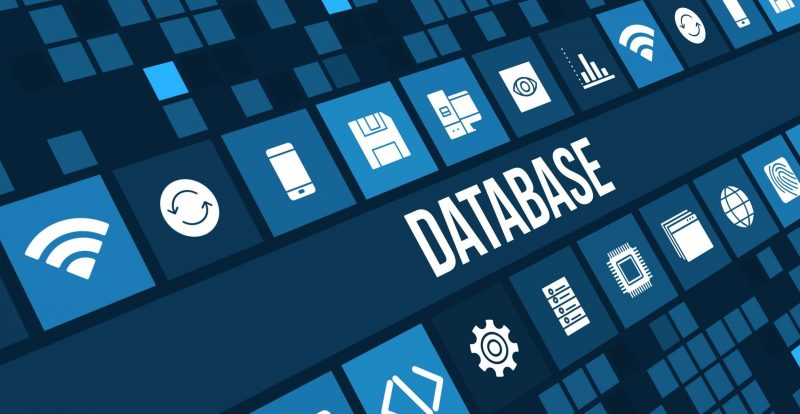
\includegraphics[scale=0.2]{images/portada}
	\end{figure}
	
\end{frame}	


% ###################   FRAME 2     ###########################

\begin{frame}

	\frametitle{2. Fundamentos de base de datos}
	
	\begin{block}{¿Qué es una base de datos?}
		Entendemos como Base de Datos un conjunto de datos estructurado y almacenado de
		forma sistemática con objeto de facilitar su posterior utilización. Una base de datos puede,
		por tanto, constituirse con cualquier tipo de datos.
	\end{block}
	
	\only<1-5>{
		 \begin{block}{Ventajas del almacenamiento estructurado}
			\begin{itemize}[<+-| alert@+>]
				\item Mayor independencia.
				\item Mayor disponibilidad.
				\item Mayor seguridad (protección de los datos).
				\item Menor redundancia.
				\item Mayor eficiencia en la captura, codificación y entrada de datos.
			\end{itemize}
		\end{block}
	}
	
	\only<6-8>{
			 \begin{block}{Resultados de la explotación de la base de datos}
				\begin{itemize}[<+-| alert@+>]
					\item \textcolor<6>{red}{Mayor coherencia.}
					\item<7-> \textcolor<7>{red}{Mayor eficiencia.}
					\item<8-> \textcolor<8>{red}{Mayor valor informativo.} 
				\end{itemize}
			\end{block}
		}		
\end{frame}

% ###################   FRAME 3     ###########################


\begin{frame}

	\frametitle{2.1 Tipos de bases de datos}
	
	\begin{enumerate} [<+-| only@+>]
		\item Modelo de base de datos plana
		\item Modelo de base de datos jeŕarquica
		\item Modelo de red
		\item Modelo de bases de datos relacionales
		\item Modelo de bases de datos NoSQL 
	\end{enumerate}
	
	\only<1>{
		\centering
		\vspace{1cm}
		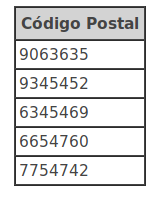
\includegraphics[scale=0.5]{images/tipo_plana}
	}
	
	\only<2>{
		\centering
		\vspace{1cm}
		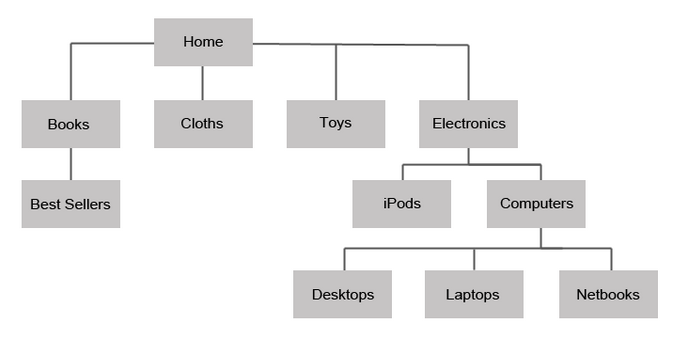
\includegraphics[scale=0.4]{images/tipo_jerarquica}
	}
	
	\only<3>{
		\centering
		\vspace{1cm}
		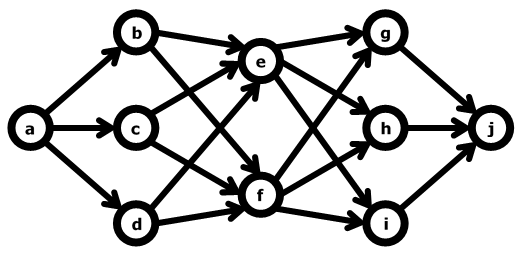
\includegraphics[scale=0.4]{images/tipo_red}
	}
	
	\only<4>{
		\centering
		\vspace{1cm}
		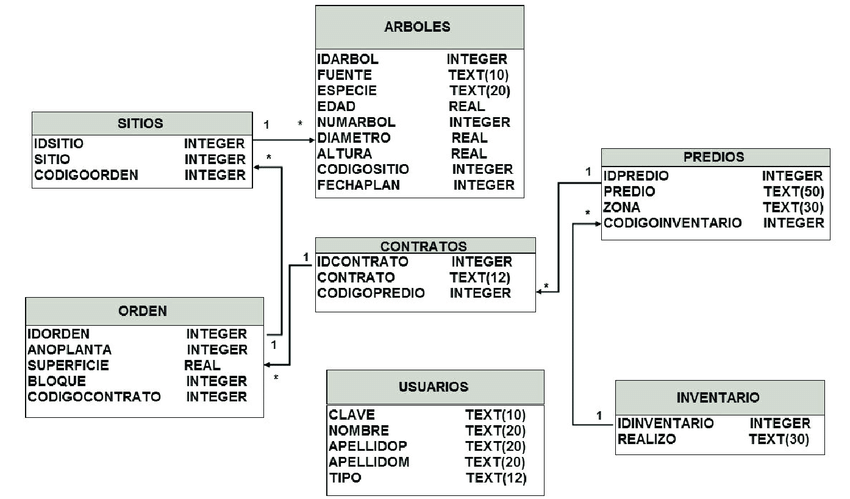
\includegraphics[scale=0.3]{images/tipo_relacional}
	}
	
	\only<5>{
		\centering
		\vspace{1cm}
		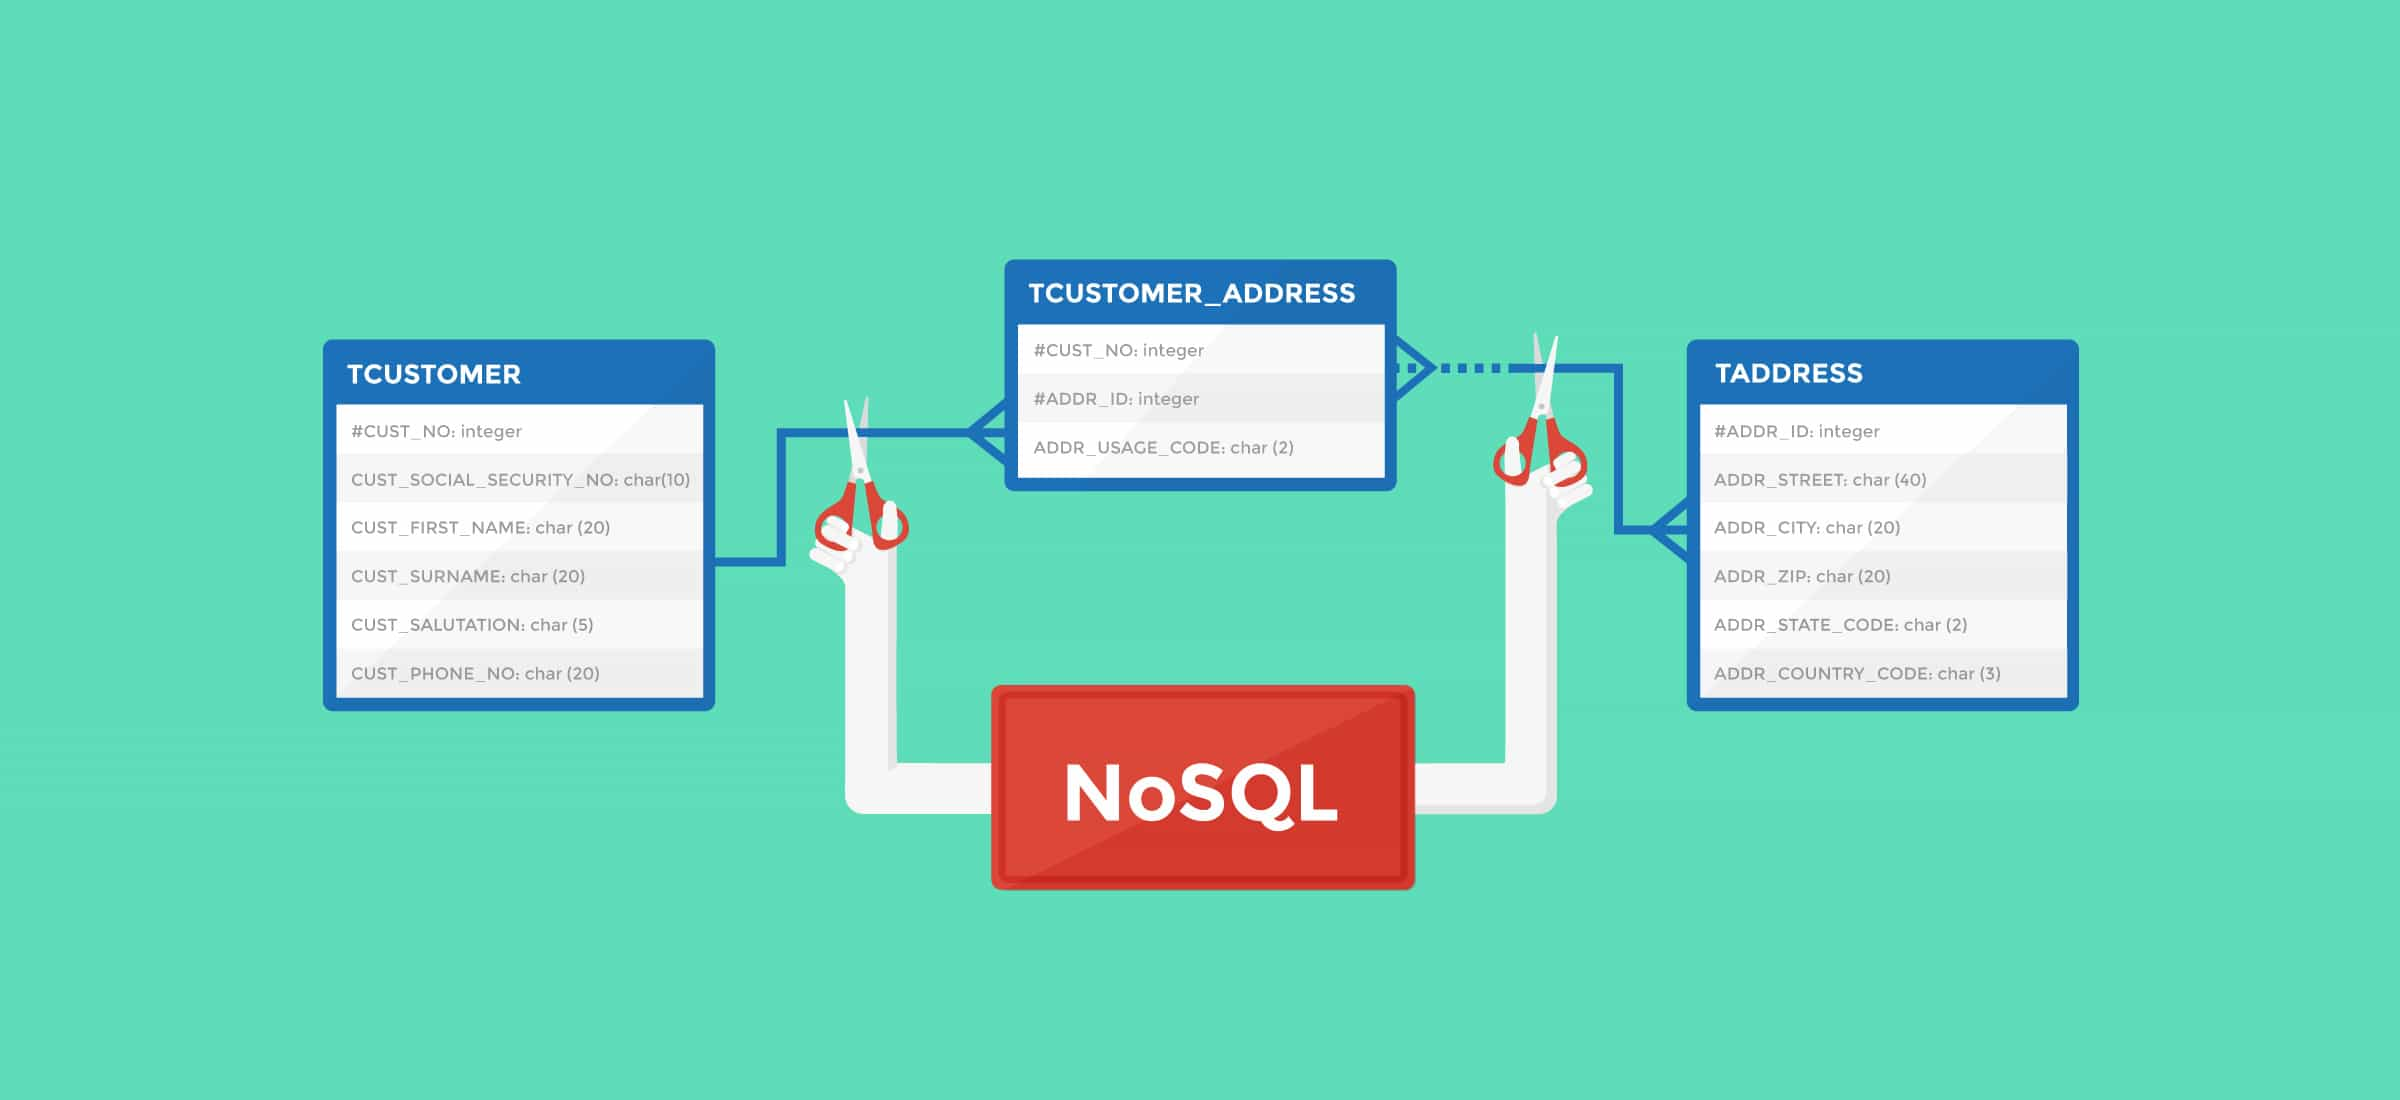
\includegraphics[scale=0.1]{images/tipo_nosql}
	}

	
\end{frame}
	
% ###################   FRAME 4     ###########################	

\begin{frame}

	\frametitle{2.2 Sistema gestor de base de datos}
	
	\begin{block}{SGBD}
		Un sistema gestor de bases de datos (SGBD) es una aplicación que permite a los
		usuarios definir, crear y mantener una base de datos, y proporciona acceso controlado a
		la misma
	\end{block}
	
	\begin{itemize}
		\item Definición de la base de datos.
		\item Inserción, actualización, eliminación y consulta de datos.
		\item Seguridad.
		\item Integridad.
		\item Concurrencia.
		\item Recuperación.
		\item Catálogos.
	\end{itemize}
	
\end{frame}
	
	
% ###################   FRAME 5     ###########################

\begin{frame}

	\frametitle{3. Bases de datos en la actualidad}
	
	Hoy en día podemos hablar sobre dos principales modelos de bases de datos: el modelo \texttt{SQL} y \texttt{NoSQL}.
	
	\only<1>{
	
		\begin{columns}
			\column{5cm}
			\vspace{1cm}
			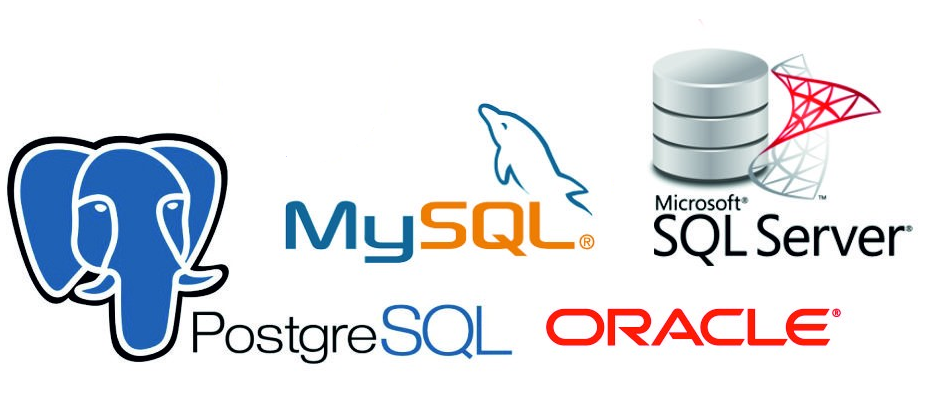
\includegraphics[scale=0.15]{images/sql}
			
			\column{6cm}
			\vspace{-1cm}
			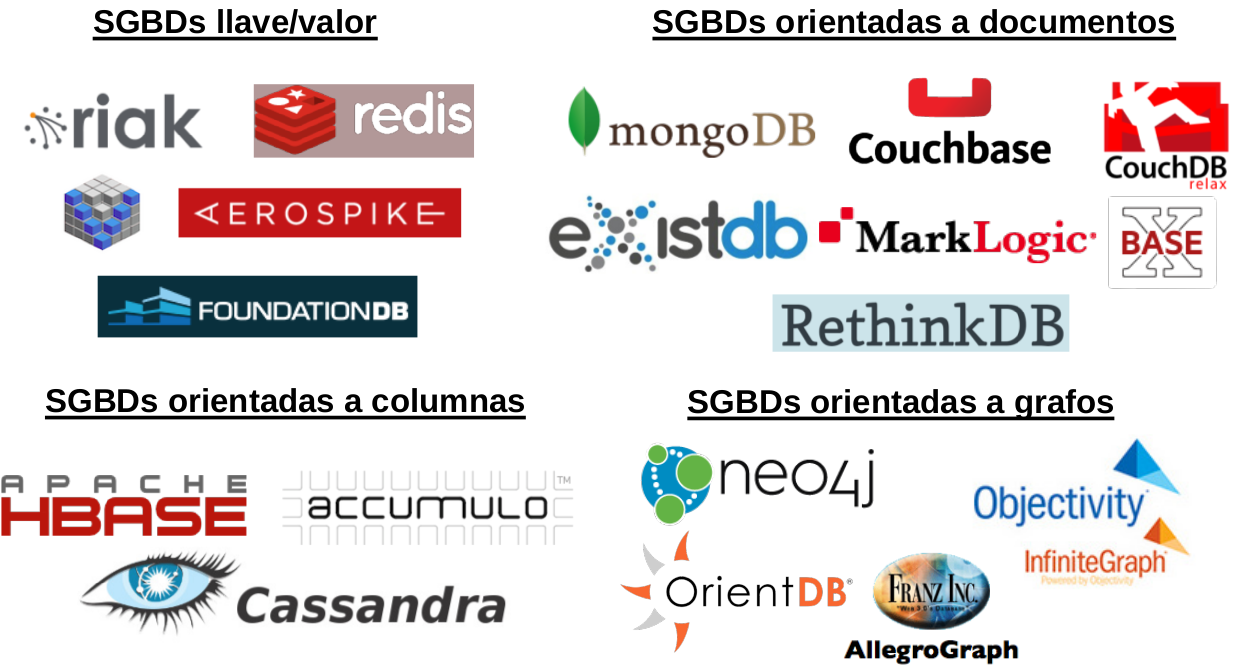
\includegraphics[scale=0.12]{images/nosql_tecnologias}
		\end{columns}
	
	}
	
	\only<2>{
		\vspace{1cm}
		\centering
		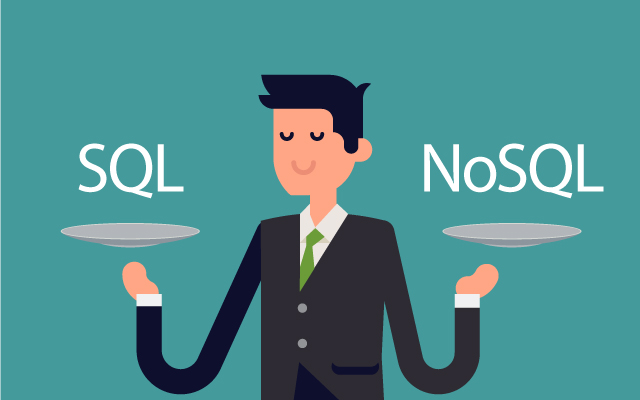
\includegraphics[scale=0.3]{images/sql_o_nosql}
	}

\end{frame}


% ###################   FRAME 6     ###########################

\begin{frame}

	\frametitle{4. Bases de datos relacionales. SQL}
	
	\begin{block}{}
		En el modelo relacional las dos capas de diseño conceptual y lógico, se parecen mucho.
		Generalmente se implementan mediante diagramas de Entidad/Relación (modelo
		conceptual) y tablas y relaciones entre éstas (modelo lógico).
	\end{block}
	
	Se rige por algunas normas sencillas
	\begin{itemize}[<+-| alert@+>]
		\item Todos los datos se representan en forma de tablas.
		\item Las tablas están compuestas por filas (o registros) y columnas (o campos) que almacenan cada uno de los registros
		\item Cada tabla debe poseer una clave primaria. Identificador único.
		\item Clave externa.
	\end{itemize}
	
\end{frame}

% ###################   FRAME 7     ###########################

\begin{frame}

	\frametitle{4. Bases de datos relacionales. SQL}
	
	\only<1>{
		Sus principales \color[rgb]{0,0.6,0}ventajas \color[rgb]{0,0,0} son:
		\begin{itemize}
			\item Mayor soporte y herramientas.
			\item Es una tecnología ampliamente conocida.
			\item Transaccionalidad entre tablas.
			\item Los datos deben cumplir con el tipo de dato definido en su estructura.	
		\end{itemize}
	}
	
	\only<2>{
		Sus principales \color[rgb]{1,0,0}inconvenientes \color[rgb]{0,0,0} son:
		\begin{itemize}
			\item Mayor soporte y herramientas.
			\item Necesita más procesamiento.
			\item La escalabilidad es reducida.	
		\end{itemize}
	}
	
	\only<3>{
		Algunas tecnologías conocidas son:
		
		\centering
		\vspace{1cm}
		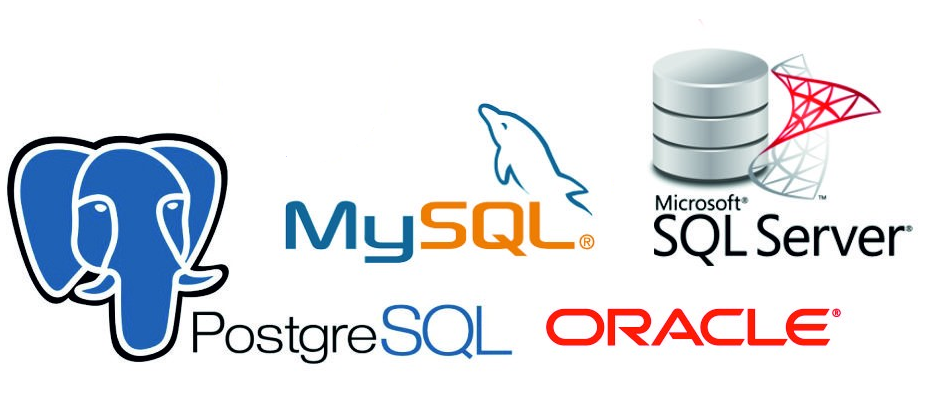
\includegraphics[scale=0.3]{images/sql}
	}
	
\end{frame}

% ###################   FRAME 7     ###########################


\begin{frame}

	\frametitle{5. Bases de datos no relacionales. NoSQL}
	
	\only<1>{
		\begin{columns}
			\column{6cm}
			\begin{block}{Bases de datos clave-valor}
				Los datos están formados en dos partes, una cadena que representa
				la clave y los datos reales a los que se hace referencia como valor, creando así un par
				“clave-valor”, que es una clave única con la que se identifica cada elemento.
			\end{block}
			
			\column{4cm}
					
			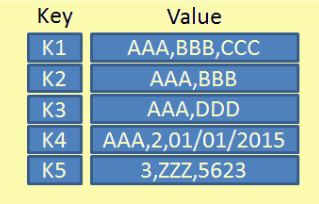
\includegraphics[scale=0.4]{images/nosql_clave-valor}
		\end{columns}
	}
	
	\only<2>{
		\begin{columns}
			\column{6cm}
			\begin{block}{Bases de datos documentales}
				Las bases de datos documentales almacenan sus datos en forma de documentos, general-
				mente utilizando como estructura JSON o XML.
			\end{block}
			
			\column{4cm}	
			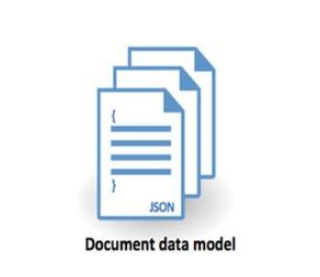
\includegraphics[scale=0.4]{images/nosql_documentos}
		\end{columns}
	}
	
	\only<3>{
		\begin{columns}
			\column{6cm}
			\begin{block}{Bases de datos orientadas a grafos}
				Las bases de datos orientadas a grafos representan las entidades como nodos de un grafo
				y las relaciones como las aristas entre ellos. Utiliza una técnica llamada adyacencia libre
				de índice (index-free adjacency) la cual consiste en que cada nodo tiene un puntero que
				apunta al nodo adyacente.
			\end{block}
			
			\column{4cm}	
			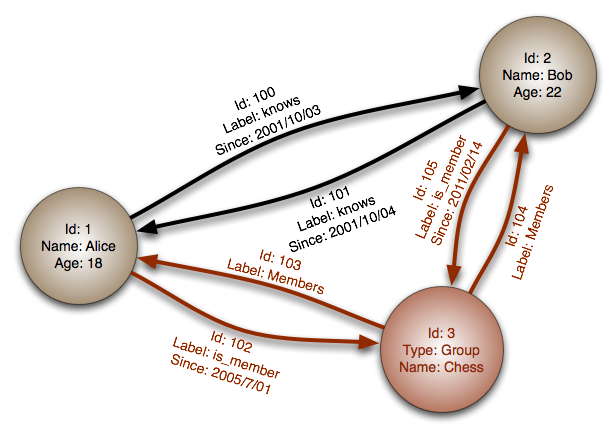
\includegraphics[scale=0.22]{images/nosql_grafos}
		\end{columns}
	}
	
	\only<4>{
		\begin{columns}
			\column{6cm}
			\begin{block}{Bases de datos orientadas a columnas}
				Son bases de datos similares a las bases de datos relacionales, aunque comparten el con-
				cepto de almacenamiento columna a columna de las bases de datos basadas en filas, los
				almacenes de columnas no almacenan los datos en tablas sino en arquitecturas distribui-
				das masivamente.
			\end{block}
			
			\column{4cm}	
			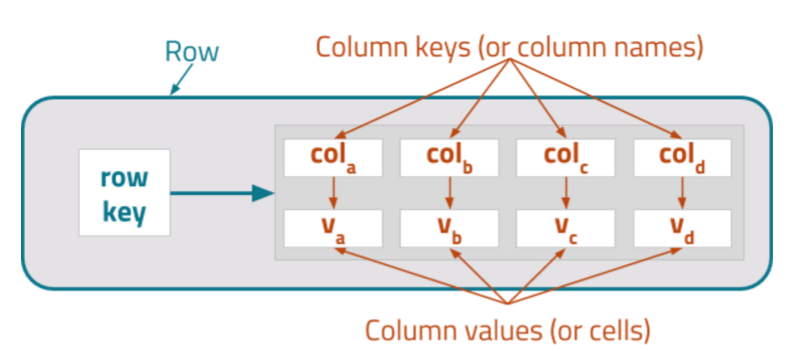
\includegraphics[scale=0.21]{images/nosql_columnas}
		\end{columns}
	}
	
	\only<5>{
		\begin{columns}
			\column{6cm}
			\begin{block}{Bases de datos orientadas a objetos}
				Son bases de datos en las cuales los datos o la información a almacenar se representan
				como un objeto (similar al de programación orientada a objetos).
			\end{block}
			
			\column{4cm}	
			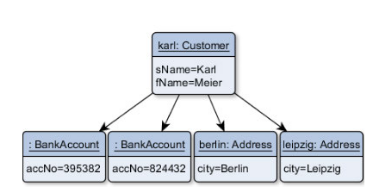
\includegraphics[scale=0.35]{images/nosql_objetos}
		\end{columns}
	}

	\only<6>{
		Las principales  \color[rgb]{0,0.6,0}ventajas \color[rgb]{0,0,0} de este modelo son:
		\begin{itemize}
			\item La \textbf{escalabilidad} y su carácter descentralizado.
			\item Suelen ser bases de datos mucho más \textbf{abiertas y flexibles}.
			\item Se pueden \textbf{hacer cambios de los esquemas} sin tener que parar bases de datos.
			\item \textbf{Escalabilidad horizontal}: son capaces de crecer en número de máquinas, en lugar
			de tener que residir en grandes máquinas.
			\item Se pueden ejecutar en \textbf{máquinas con pocos recursos}.
			\item \textbf{Optimización de consultas} en base de datos para grandes cantidades de datos.
		\end{itemize}
	}
	
	\only<7>{
			Los principales \color[rgb]{1,0,0}inconvenientes \color[rgb]{0,0,0} de este modelo son:
			\begin{itemize}
				\item No todas las bases de datos NoSQL contemplan la \textbf{atomicidad} de las instrucciones
				y la \textbf{integridad de los datos}.
				\item Problemas de \textbf{compatibilidad entre instrucciones SQ}L.
				\item Falta de \textbf{estandarización}.
				\item Soporte \textbf{multiplataforma}.
				\item \textbf{herramientas} de administración \textbf{no muy usables}.
			\end{itemize}
		}
\end{frame}

% ###################   FRAME 8     ###########################

\begin{frame}

\frametitle{6. Comparativa SQL vs NoSQL}

	\only<1>{
	
		\begin{columns}
			\column{5cm}
			\begin{block}{¿Es NoSQL el sustituto directo para evolucionar de las antiguas bases de datos
				relacionales?}
				Esto no es cierto para todos los casos, sino que se tiene que tener en cuenta
				el diseño del problema para poder saber a qué modelo de base de datos se puede ajustar
				mejor.
			\end{block}
			
			\column{6cm}
			\vspace{-1cm}
			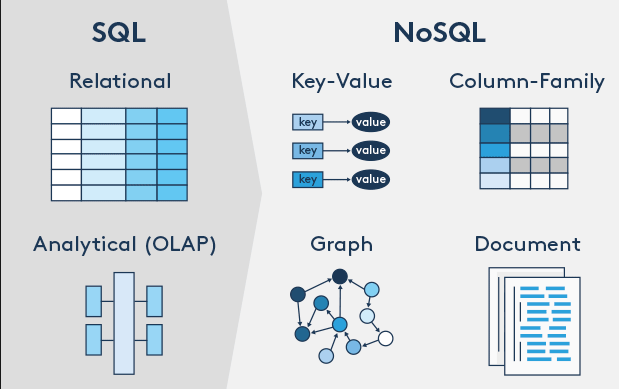
\includegraphics[scale=0.25]{images/comparativa_sql_vs_nosql}
		\end{columns}
	
	}
	\only<2>{
		\begin{block}{Integridad de datos}
			\textbf{SQL}:Las tablas tienen estructuras rígidas, donde cada dato tiene un tipo definido,
			no podemos almacenar datos de otro tipo diferente, y no se vale más de un dato en
			un mismo campo.
			\vspace{0.4cm}
			
			\textbf{NoSQL}:Hay varios tipos de base de datos NoSQL, pero en general, ninguna te exige
			que definas el tipo de datos que vas a almacenar.
		\end{block}
	}
	
	\only<3>{
		\begin{block}{Operaciones atómicas}
			\textbf{SQL}:Las bases de datos relacionales tienen atomicidad gracias a que sus tablas
			están conectadas y pueden “ponerse de acuerdo” para no aceptar cambios nuevos
			hasta que termine una transacción.
			\vspace{0.4cm}
			
			\textbf{NoSQL}:Datos no relacionales = no hay relaciones sobre las que hacer una transacción atómica. Simplemente, cuando quieres hacer cambios en 5 entidades diferentes,
			de frente o detrás de cámaras habrá 5 llamadas diferentes a la base de datos una
			detrás de otra..
		\end{block}
	}
	
	\only<4>{
		\begin{block}{Escalabilidad}
			\textbf{SQL}:La verdad es que la mayoría de soluciones SQL tienen buen soporte para
			escalar verticalmente.
			\vspace{0.4cm}
			
			\textbf{NoSQL}:Cuando no tienes la consistencia de datos como prioridad, distribuir y
			replicar tu base de datos en múltiples máquinas es trivial, y por eso se considera
			que el NoSQL es excelente para bases de datos necesitan escalar horizontalmente.
		\end{block}
	}
	
	\only<5>{
		\begin{block}{Velocidad}
			\textbf{SQL}:Las garantías que te dan las relaciones conllevan un precio. Esto es más evidente cuando empezamos a hacer consultas con “joins” (que involucran múltiples
			entidades) y de repente una búsqueda puede tardar minutos y hasta horas
			debido a la gran cantidad de datos que está revisando.
			\vspace{0.4cm}
			
			\textbf{NoSQL}:Las bases de datos no relacionales suelen contar con mecanismos de búsqueda sumamente rápida para	conseguir un dato específico entre millones.
		\end{block}
	}
	\only<6>{
		\begin{block}{Consistencia vs redundancia}
			\textbf{SQL}:La consistencia de datos es asegurarse de que un único dato este una única
			vez en toda la base de datos; y se suele lograr con el proceso de “Normalización”.
			\vspace{0.4cm}
			
			\textbf{NoSQL}:La redundancia es repetir adrede los datos a conveniencia en varias partes
			de la BD.
		\end{block}
	}
	
	\only<7>{
		\begin{block}{Comodidad para el desarrollador}
			\textbf{SQL}:La comunidad SQL lleva décadas madurando, y esto se traduce no solo en
			mejores herramientas administrativas, sino en estándares mejores definidos, mayor
			documentación.
			\vspace{0.4cm}
			
			\textbf{NoSQL}:Aquí el punto fuerte es la conveniencia: factores como que los datos no necesiten tipos o que puedas aprovechar la redundancia, hacen más flexible el desarrollar con NoSQL.
		\end{block}
	}
	
	\only<8>{
		\begin{table}[H]
			\centering
			\begin{tabular}[c]{|l |l |l|}
				\hline
				\rowcolor{azulOscuro} \color{white}Característica & \color{white}NoSQL & \color{white}SQL \\
				\hline
				\cellcolor{azulClaro} Rendimiento & \cellcolor{verdeSuave}Alto & \cellcolor{rojoSuave}Bajo \\
				\cellcolor{azulClaro}Confiabilidad & \cellcolor{rojoSuave}Baja & \cellcolor{verdeSuave}Buena \\
				\cellcolor{azulClaro}Disponibilidad & \cellcolor{verdeSuave}Buena & \cellcolor{verdeSuave}Buena \\
				\cellcolor{azulClaro}Consistencia & \cellcolor{rojoSuave}Baja & \cellcolor{verdeSuave}Buena \\
				\cellcolor{azulClaro}Almacenamiento & \cellcolor{verdeSuave}Enormes cantidades & \cellcolor{amarilloSuave}Cantidades medio/grande \\
				\cellcolor{azulClaro}Escalabilidad & \cellcolor{verdeSuave}Alta & \cellcolor{amarilloSuave}Alta pero más cara \\
				\hline
			
			\end{tabular}
			\caption{Resumen de las características NoSQL y SQL}
		\end{table}
		
	}
		
\end{frame}

% ###################   FRAME 9     ###########################

\begin{frame}
	
	\frametitle{7. Conclusiones}
	
	Muchas personas piensan que las tecnologías NoSQL son lo “nuevo” y por lo tanto todo
	debe migrar a este modelo, pero es un grave error. NoSQL no es un reemplazo, es simplemente un modelo diferente que ofrece ventajas y soluciones a problemas que poseen
	las bases de datos relacionales.
	
	\begin{block}{SQL}
		\begin{itemize}
			\item Respeto por la integridad de los datos.
			\item Si se necesita información con estructura consistente.
			\item Si la jerarquía de datos es importante\ldots
		\end{itemize}
	\end{block}
	
	\begin{block}{NoSQL}
			\begin{itemize}
				\item Si la escalabilidad es importante.
				\item Si no es necesario respetar la integridad de los datos.
				\item Desarrollo Big data.
			\end{itemize}
		\end{block}
	
\end{frame}

% ###################   FRAME 10     ###########################

\begin{frame}
	\LARGE
	\centering
	\textbf{Gracias por su atención}
	\large 
	
	Para más información se puede consultar el repositorio en github.
	
	\begin{columns}
		\column{3cm}
		\centering
		
\includegraphics[scale=0.1]{images/github}
		
		
		\column{8cm}
		\small
		 \color[rgb]{0,0,1} \url{https://github.com/jmv74211/LaTeX/tree/master/ejercicios/Entrega\_final}
				
	\end{columns}
	
	\vspace{1cm}
	
\includegraphics[scale=0.2]{images/logo_ugr}

\end{frame}

\end{document}